\section{Classical Algorithms}
In this section, we will take a look at each of the components of the blockchain implemented classically.
\subsection{Encryption}
Encryption is used to digitally sign transactions in a blockchain. Encryption is the process by which data is converted into a secure string of bits that can be uniquely decrypted. Encryption requires the use of a private key to decrypt an encrypted message and a public key to verify the encryption. Several encryption algorithms exists in the market, the most popular ones being the 3DES, AES and RSA\cite{enc_rsa}. 
\subsection{Hashing}
Hashing is the process by which a message of arbitrary lengths is converted to a bit string of fixed length. Unlike encryption, hashes are not unique. Several messages can have the same hash. Hashes must be easy to verify given a message. The reverse process, however, should be a hard one, i.e., given a hash, it should be practically impossible to find a message generating the hash. Hash collisions should also be rare, i.e., given a message and its hash, it should be practically impossible to find another message with the same hash. Finally, hashes must be distinctly different even for change of a single character in the message. Some commonly used hashing algorithms include SHA-1, Pearson Hash and SHA-256. In this paper, we will demonstrate the SHA-256. We will then design a surrogate hashing purpose that satisfies the aforementioned properties of hashes but is easy to simulate on a quantum computer.
\subsubsection*{SHA-256}
This comprises using XOR and shift operators on registers pre-loaded with existing values. The code for the same is mentioned below. The code is written in python.
\begin{lstlisting}
import math
import numpy as np

#The first 32 prime numbers are used to preset the hash registers by considering the fractional part of their square and cube roots
PRIMES=[2, 3, 5, 7, 11, 13, 17, 19, 23, 29, 31, 37, 41, 43, 47, 53, 59, 61, 67, 71, 73, 79, 83, 89, 97, 101, 103, 107, 109, 113, 127, 131, 137, 139, 149, 151, 157, 163, 167, 173, 179, 181, 191, 193, 197, 199, 211, 223, 227, 229, 233, 239, 241, 251, 257, 263, 269, 271,277,281,283,293,307,311]

#Right shift by n bits
def SHR_int(x,n):
    return x>>n
def SHR(s,n):
    x=int(s,2)
    return str(bin(x>>n))[2:].zfill(32)

#Right rotate by n bits
def ROTR_int(x,n):
    return (x>>n)|(x<<(32-n))&0xFFFFFFFF
def ROTR(s,n):
    x=int(s,2)
    return str(bin((x>>n)|(x<<(32-n))&0xFFFFFFFF))[2:].zfill(32)

#Linear combination in terms of XOR
def SIG0(x):
    return ROTR_int(x,2)^ROTR_int(x,13)^ROTR_int(x,22)
def SIG1(x):
    return ROTR_int(x,6)^ROTR_int(x,11)^ROTR_int(x,25)
    #return x
def sig0(s):
    x=int(s,2)
    return str(bin(ROTR_int(x,7)^ROTR_int(x,18)^SHR_int(x,3)))[2:].zfill(32)
def sig1(s):
    x=int(s,2)
    return str(bin(ROTR_int(x,17)^ROTR_int(x,19)^SHR_int(x,10)))[2:].zfill(32)
def che(x,y,z):
    return (x&y)|(~x&z)
def maj(x,y,z):
    return (x&y)^(y&z)^(z&x)

#Converts message to ASCII
def toAscii(message):
    return ''.join(str(bin(ord(c)))[2:].zfill(8) for c in message)

#Pads the message with zeroes till length is a multiple of 512 and then appends the length at the end
def padding(message_ascii):
    l=len(message_ascii)
    size=(l//512+1)*512
    pad=message_ascii+'1'
    for j in range(size-len(pad)-64):
        pad=pad+'0'
    pad=pad+str(bin(len(toAscii(message))))[2:].zfill(64)
    return pad,size

#Creates the message block
def message_block(message):
    padded_message=padding(toAscii(message))[0]
    nblocks=padding(toAscii(message))[1]//512
    w=[[None for _ in range(64)] for _ in range(nblocks)]
    for i in range(nblocks):
        for j in range(16):
            w[i][j]=padded_message[512*i+32*j:512*i+32*(j+1)]
        for j in range(16,64):
            w[i][j]=str(bin((int(sig1(w[i][j-2]),2)+int(w[i][j-7],2)+int(sig0(w[i][j-15]),2)+int(w[i][j-16],2))%int(2**32)))[2:].zfill(32)
    return w

#Compression where registers are continuously updated with values of the linear functions above to generate the hash
def compress(w,H0):
    H=H0
    for j in range(len(w)):
        wj=int(w[j],2)
        T1=(K[j]+wj+SIG1(H[4])+che(H[4],H[5],H[6])+H[7])%int(2**32)
        T2=(SIG0(H[0])+maj(H[0],H[1],H[2]))%int(2**32)  
        H=[(T1+T2)%int(2**32) ]+H[:-1]
        H[4]=(H[4]+T1)%int(2**32)
    return [(H0[i]+H[i])%int(2**32) for i in range(len(H))]

#Generates the hash in hexadecimal
def hashgen(message,H0):
    w=message_block(message)
    H=H0
    for i in range(len(w)):
        H=compress(w[i],H)
    return ''.join(str(hex(x))[2:].zfill(8) for x in H)

#Actually initializing the registers
K=[]
H=[]
for i in range(64):
    K.append(int(math.modf((PRIMES[i])**(1/3))[0]*(2**32)))
for i in range(8):
    H.append(int(math.modf((PRIMES[i])**(1/2))[0]*(2**32)))

#Inputiing the message from the user
message=input().rstrip()
#Printing the hash
print(hashgen(message,H))
\end{lstlisting}
Now we shall check the values of the hash for some sample strings. This can be done by running the code given above.\\
Message: \verb|Hello World|\\
Hash: \verb|a591a6d40bf420404a011733cfb7b190d62c65bf0bcda32b57b277d9ad9f146e|\\
Making a slight change\\
Message: \verb|Hello Workd|\\
Hash: \verb|5ab45e33f10c8c9eb8005ba117fbd6e9d4ce3e61d5b199c08cbb7bbebf58cf68|\\
We see that the hash changes significantly.
\subsubsection*{Surrogate Hash Function: Pearson Hashes and LFSRs}
The SHA-256 is a rather cumbersome method of hashing that requires significant amount of time and memory when simulating using qiskit. To overcome this difficulty, we will use a surrogate hash called the Pearson Hash\cite{pearson}. The Pearson Hash makes use of a lookup table, which can be achieved using Linear Feedback Shift Registers (LFSR)\cite{lfsr}. These are easy to implement in qiskit\cite{qlfsr}, and the hash so generated satisfies the properties of a good hash. Since the purpose of our project is the search for nonce for a given hashing algorithm and not hashing, using a surrogate hashing algorithm will make no difference.

An LFSR comprises shift registers in which, at each iteration, the elements shift to the adjacent register (like in an ordinary shift register) and the first register takes the value of a linear function of some of the registers. Galois Theory of Fields dictates the working of these LFSRs (See \ref{appA}). The values which are XORed are called taps.
The LFSR structure is shown in Figure \ref{Fig:3}
where $\oplus$ denotes XOR.
\begin{figure}[!htb]
   \begin{minipage}{\textwidth}
     \centering
     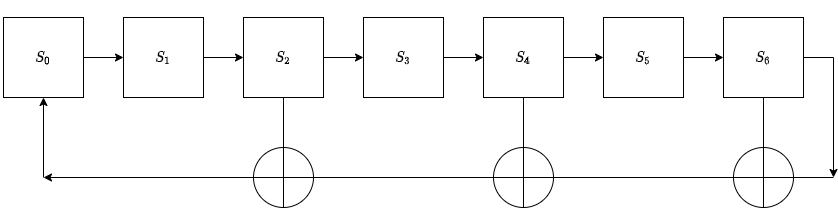
\includegraphics[width=1\linewidth]{fig3.png}
     \caption{A sample LFSR with taps at 2,4 and 6}
     \label{Fig:3}
   \end{minipage}
\end{figure}

Pearson hashing uses two LFSRs. It works by taking the XOR of a character with the register and then performing two different sets of LFSRs. While LFSRs by themselves are reversible, it is impossible to extract the characters of a message from the hashing owing to the repeated XOR operations.
\subsection{The Epoch, Nonce and Mining}
The time stamp appended in a block (see \ref{Fig:1}) is called an epoch. It is a 4-byte integer that represents the number of seconds passed from January 1, 1970 00:00 UTC.\\
The nonce is the arbitrary string that needs to be found by brute force algorithms to ensure the hash starts with a certain minimum number of zeroes. The process of finding the nonce is called "mining" in the language of crypto-currencies. Mining requires heavy use of resources like electricity and computing power. Bitcoin miners are often provided with incentives for the process. Since we have a 256-bit hash, mining success probability is of the order of $2^{-256}$, a number that is astronomically small. Mining is a form of proof of work that ensures fraudulent individuals do not take advantage of a decentralized ledger. If the majority mines honest blocks, it becomes easy for someone or the other to get the nonce. In case of a fork in terms of two different blockchains with appropriate nonces, the longer blockchain gets accepted.\\
The hash function that we are using generates 8-bit long hashes. Our nonce can thus be 8-bit long, which can be represented by a single character.